\documentclass[11pt]{amsart}

\usepackage[T1]{fontenc}
\usepackage{lmodern}
\usepackage{amssymb,amsmath}
\usepackage{graphicx}
\usepackage{booktabs}
\usepackage{array}
\usepackage{xcolor}
\usepackage[margin=1.15in]{geometry}
\usepackage[colorlinks=true,linkcolor=blue!50!black,citecolor=blue!50!black,urlcolor=blue!50!black]{hyperref}

\newtheorem{theorem}{Theorem}[section]
\newtheorem{proposition}[theorem]{Proposition}
\newtheorem{lemma}[theorem]{Lemma}
\newtheorem{corollary}[theorem]{Corollary}
\newtheorem*{maintheorem}{Theorem}
\theoremstyle{definition}
\newtheorem{definition}[theorem]{Definition}
\newtheorem{question}[theorem]{Question}
\theoremstyle{remark}
\newtheorem{remark}[theorem]{Remark}

\numberwithin{equation}{section}
\raggedbottom

\newcommand{\doi}[1]{\href{https://doi.org/#1}{\nolinkurl{doi:#1}}}
\newcommand{\Z}{\mathbb{Z}}
\newcommand{\NN}{\operatorname{N}}
\newcommand{\ind}[1]{[\,#1\,]}
\hypersetup{pdftitle={The book Ramsey number R(B57,B58)=231},pdfauthor={Deep Bhattacharjee}}

\begin{document}

\title[The book Ramsey number $R(B_{57},B_{58})=231$]{The book Ramsey number $R(B_{57},B_{58})=231$}

\author{Deep Bhattacharjee}
\address{Formerly, Electro-Gravitational Space Propulsion Laboratory (EGSPL),\newline Bhubaneswar, Odisha 751030, India}
\email{d.bhattacharjee@erl-forschung.de}
\email{itsdeep@live.com}
\urladdr{https://orcid.org/0000-0003-0466-750X}
\thanks{Corresponding author: \href{mailto:d.bhattacharjee@erl-forschung.de}{d.bhattacharjee@erl-forschung.de}; ORCID \href{https://orcid.org/0000-0003-0466-750X}{\mbox{0000-0003-0466-750X}}}

\subjclass[2020]{Primary 05C55; Secondary 05C25, 05B10}
\keywords{Ramsey number, book graph, block-circulant graph}

\begin{abstract}
We construct a graph on $230$ vertices with no book $B_{57}$ whose complement contains no $B_{58}$. With the upper bound of Rousseau and Sheehan this gives $R(B_{57},B_{58})=231$, the smallest case of Wesley's conjecture $R(B_{n-1},B_n)=4n-1$ that was open. The graph is a two-block circulant graph over $\Z_{115}$, and the proof reduces to $57$ inequalities.
\end{abstract}

\maketitle

\section{Introduction}

The book $B_k$ is the graph $K_2+\overline{K_k}$: $k$ triangles sharing one edge, its spine. For graphs $G$ and $H$, the Ramsey number $R(G,H)$ is the least $N$ such that every graph on $N$ vertices contains $G$ or has a complement containing $H$. Rousseau and Sheehan~\cite{RS} proved, from Goodman's count of monochromatic triangles~\cite{Go}, that
\begin{equation}\label{eq:RS}
R(B_{n-1},B_n)\le 4n-1\qquad(n\ge2).
\end{equation}
Wesley~\cite{We} proved equality for $n\le20$ and whenever $2n-1$ is a prime power congruent to $1$ modulo $4$, and conjectured equality for every $n$; the conjecture is one of the open problems of Epoch AI's FrontierMath collection~\cite{Ep}. Turturean~\cite{Tu} constructed extremal graphs for every $n\le57$ and for fourteen further values below $100$, partly through a cyclotomic construction of Szekeres~\cite{Sz}; Chung, Du and Wesley~\cite{CDW} found three further infinite families and settled $n=67$ by a finite certificate~\cite{CDWd}, for which~\cite{Bh} gives a proof checkable by hand; and Price obtained $n=70$~\cite{Ep}. Before the present note the smallest open case was $n=58$.\footnote{The values $n\le100$ that none of the constructions cited here covers were $58$, $59$, $60$, $64$, $65$, $68$, $72$, $73$, $76$, $78$, $80$, $81$, $84$, $88$, $89$, $92$, $93$, $94$, $96$ and $100$. This list is our reading of~\cite{CDW,CDWd,Ep,Tu,We} as of 15 October 2026; it agrees with the ledger in~\cite[Section~6.1]{CDWd}.}

\begin{maintheorem}
$R(B_{57},B_{58})=231$.
\end{maintheorem}

The upper bound is~\eqref{eq:RS}, and the lower bound is a graph on $230$ vertices with no $B_{57}$ whose complement has no $B_{58}$. For odd $n$ the graph of~\cite{Bh} and the Paley graphs of~\cite{We} are regular two-block circulant graphs over $\Z_{2n-1}$ whose two blocks are complementary circulants of degree $n-1$. When $n$ is even such a graph does not exist, because a symmetric subset of $\Z_{2n-1}\setminus\{0\}$ has even size. Turturean's examples for even $n$~\cite{Tu} enlarge the first block by one element and shrink the second by one, and our graph has that shape. Section~\ref{sec:blocks} reduces the two book conditions for it to one inequality~\eqref{eq:star} on the connection sets, a reduction that underlies the search of~\cite{Tu} and that we prove here in full. Section~\ref{sec:58} gives the connection sets for $n=58$, and Table~\ref{tab:main} verifies~\eqref{eq:star} at the $57$ values of $d$ that matter. The graph has also been checked by two independent programs and in Lean~4 (see the end of the paper).

\section{Two-block circulant graphs of even order}\label{sec:blocks}

Throughout, $n\ge4$ is even, $v=2n-1$ and $G=\Z_v$. For $X,Y\subseteq G$ and $d\in G$ put
\[
\NN_{X,Y}(d)=|X\cap(Y+d)|=\#\{y\in Y:\ y+d\in X\}.
\]
Translating by $-d$ shows $\NN_{X,X}(-d)=\NN_{X,X}(d)$, and $\sum_{d\in G}\NN_{X,X}(d)=|X|^2$.

Let $A\subseteq G\setminus\{0\}$ with $A=-A$ and $|A|=n$, let $C=G\setminus(A\cup\{0\})$, so that $C=-C$ and $|C|=n-2$, and let $B\subseteq G$ with $|B|=n-1$. The graph $\Gamma=\Gamma(A,B)$ has vertex set $G\times\{0,1\}$, and
\[
(x,0)\sim(y,0)\iff y-x\in A,\qquad (x,1)\sim(y,1)\iff y-x\in C,
\]
and $(x,0)\sim(y,1)$ if and only if $y-x\in B$. Since $A$ and $C$ are symmetric and avoid $0$, $\Gamma$ is a simple graph on $4n-2$ vertices. A vertex $(x,0)$ has $|A|+|B|=2n-1$ neighbours and a vertex $(x,1)$ has $|C|+|B|=2n-3$; the translations $(x,i)\mapsto(x+t,i)$ are automorphisms. Write $\lambda(p,q)$ for the number of common neighbours of two vertices, $\mu(p,q)$ for the number of vertices other than $p$ and $q$ adjacent to neither, $\ind{P}$ for the indicator of a statement $P$, and
\[
f(d)=\NN_{A,A}(d)+\NN_{B,B}(d)\qquad(d\in G).
\]

\begin{lemma}\label{lem:lambda}
For $d\ne0$,
\[
\lambda\big((0,0),(d,0)\big)=f(d),\qquad \lambda\big((0,1),(d,1)\big)=f(d)-3+2\ind{d\in A},
\]
and for every $d\in G$, $\lambda\big((0,0),(d,1)\big)=n-1-\ind{d\in B}$.
\end{lemma}

\begin{proof}
A vertex $(z,0)$ is a common neighbour of $(0,0)$ and $(d,0)$ when $z\in A$ and $z-d\in A$, and $(z,1)$ is one when $z\in B$ and $z-d\in B$; this gives $\NN_{A,A}(d)+\NN_{B,B}(d)$.

For $(0,1)$ and $(d,1)$, the common neighbours $(z,1)$ are counted by $\NN_{C,C}(d)$. A vertex $(z,0)$ is adjacent to $(0,1)$ when $-z\in B$ and to $(d,1)$ when $d-z\in B$; with $w=-z$ these say $w\in B$ and $w+d\in B$, so there are $\NN_{B,B}(-d)=\NN_{B,B}(d)$ of them. To compute $\NN_{C,C}(d)$, let $S=A\cup\{0\}$, so that $|S|=n+1$ and $C=G\setminus S$. Then $|C\cap(C+d)|=v-|S\cup(S+d)|=v-2(n+1)+|S\cap(S+d)|$. The set $S\cap(S+d)$ is the disjoint union of $A\cap(A+d)$, of $\{0\}$ when $-d\in A$, and of $\{d\}$ when $d\in A$; neither $0$ nor $d$ lies in $A\cap(A+d)$, because $0\notin A$. As $A=-A$ and $v-2(n+1)=-3$, we get $\NN_{C,C}(d)=\NN_{A,A}(d)-3+2\ind{d\in A}$.

For $(0,0)$ and $(d,1)$, a vertex $(z,0)$ is a common neighbour when $z\in A$ and $d-z\in B$, that is, $z=d-b$ with $b\in B$ and $d-b\in A$; since $A=-A$ the last condition reads $b-d\in A$. A vertex $(z,1)$ is a common neighbour when $z\in B$ and $z-d\in C$. Together, $\lambda=\#\{b\in B:\ b-d\in A\cup C\}=\#\{b\in B:\ b\ne d\}=n-1-\ind{d\in B}$.
\end{proof}

\begin{lemma}\label{lem:mu}
Let $p,q$ be distinct non-adjacent vertices of $\Gamma$. Then $\mu(p,q)=\lambda(p,q)-2$ if both lie in $G\times\{0\}$, $\mu(p,q)=\lambda(p,q)+2$ if both lie in $G\times\{1\}$, and $\mu(p,q)=\lambda(p,q)$ otherwise.
\end{lemma}

\begin{proof}
The neighbourhoods of $p$ and $q$ lie among the other $4n-4$ vertices, and their union has $\deg p+\deg q-\lambda(p,q)$ elements, so $\mu(p,q)=4n-4-\deg p-\deg q+\lambda(p,q)$. Insert the degrees $2n-1$ and $2n-3$.
\end{proof}

\begin{proposition}\label{prop:star}
$\Gamma(A,B)$ contains no $B_{n-1}$ and its complement contains no $B_n$ if and only if
\begin{equation}\label{eq:star}
f(d)\le n+1-3\,\ind{d\in A}\qquad\text{for every } d\in G\setminus\{0\}.
\end{equation}
In that case $R(B_{n-1},B_n)=4n-1$.
\end{proposition}

\begin{proof}
An edge lying in $k$ triangles is the spine of a $B_k$, and a non-edge $pq$ is the spine of a $B_k$ in the complement exactly when $\mu(p,q)\ge k$. So the two conditions say that $\lambda(p,q)\le n-2$ for every edge and $\mu(p,q)\le n-1$ for every pair of distinct non-adjacent vertices. By translation it suffices to take $p=(0,i)$, and we use Lemmas~\ref{lem:lambda} and~\ref{lem:mu}.

For $p=(0,0)$ and $q=(d,0)$ with $d\ne0$, the pair is an edge if and only if $d\in A$. For $d\in A$ the condition is $f(d)\le n-2$, and for $d\notin A$ it is $f(d)-2\le n-1$; together they are~\eqref{eq:star}. For $p=(0,1)$ and $q=(d,1)$, the pair is an edge if and only if $d\in C$, that is, $d\notin A$. For $d\notin A$ the condition is $f(d)-3\le n-2$, and for $d\in A$ it is $(f(d)-1)+2\le n-1$; together they are again~\eqref{eq:star}. For $p=(0,0)$ and $q=(d,1)$ the pair is an edge if and only if $d\in B$; then $\lambda=n-2$, and otherwise $\mu=\lambda=n-1$, so the condition holds with equality in both cases. The pairs $(0,1),(d,0)$ are translates of these. The last sentence follows from~\eqref{eq:RS}, since $\Gamma$ has $4n-2$ vertices.
\end{proof}

\begin{remark}\label{rem:slack}
Summing over $d\ne0$ gives $\sum f(d)=n(n-1)+(n-1)(n-2)=2(n-1)^2$ and $\sum\big(n+1-3\ind{d\in A}\big)=(n+1)(2n-2)-3n=(n-2)(2n+1)$. So when~\eqref{eq:star} holds, the slacks $s(d)=n+1-3\ind{d\in A}-f(d)$ are non-negative integers with sum $n-4$, and~\eqref{eq:star} is an equality for at least $n+2$ of the $2n-2$ values of $d$. For the regular graphs used when $n$ is odd~\cite{Bh,We} the corresponding sum is $n-1$, so the even case is tighter. The cross pairs never matter: $B$ enters only through its autocorrelation $\NN_{B,B}$. Since $f(-d)=f(d)$ and $\ind{-d\in A}=\ind{d\in A}$, it suffices to check~\eqref{eq:star} for $1\le d\le n-1$.
\end{remark}

\section{The case \texorpdfstring{$n=58$}{n = 58}}\label{sec:58}

Let $n=58$ and $v=115=5\cdot23$. Let $A=\pm A_+$ and let $B$ be the sets
\begin{align*}
A_+=\{&3, 10, 11, 14, 16, 18, 21, 23, 24, 25, 26, 27, 28, 29, 30, 32, 36, 37, 38, 43, 44, 46, 47,\\
&48, 49, 52, 54, 55, 56\},\\
B=\{&0, 2, 5, 6, 7, 9, 10, 11, 15, 17, 20, 21, 22, 23, 24, 26, 30, 34, 38, 43, 44, 46, 47, 50, 52,\\
&53, 54, 56, 59, 65, 66, 67, 69, 71, 72, 73, 74, 75, 80, 81, 83, 84, 85, 88, 90, 92, 93, 97,\\
&100, 102, 105, 106, 107, 109, 110, 111, 114\}.
\end{align*}
The $29$ elements of $A_+$ lie in $\{1,\dots,57\}$, so $A=A_+\cup(-A_+)$ has $58$ elements, avoids $0$ and satisfies $A=-A$; and $|B|=57$. Written out,
\begin{align*}
A=\{&3, 10, 11, 14, 16, 18, 21, 23, 24, 25, 26, 27, 28, 29, 30, 32, 36, 37, 38, 43, 44, 46, 47,\\
&48, 49, 52, 54, 55, 56, 59, 60, 61, 63, 66, 67, 68, 69, 71, 72, 77, 78, 79, 83, 85, 86, 87,\\
&88, 89, 90, 91, 92, 94, 97, 99, 101, 104, 105, 112\}.
\end{align*}
Figure~\ref{fig:torus} draws both sets on the torus $\Z_5\times\Z_{23}$.

\begin{figure}[t]
\centering
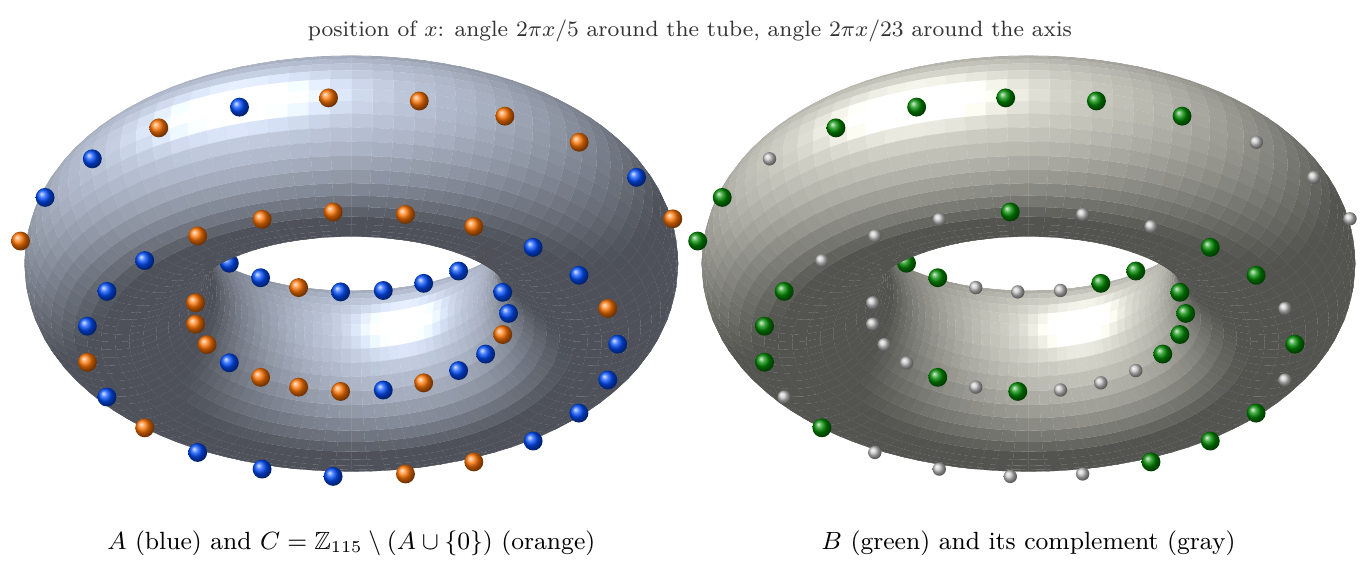
\includegraphics[width=\textwidth]{figures/torus.png}
\caption{The sets $A$ and $B$ for $n=58$. The residue $x\in\Z_{115}$ sits at angle $2\pi x/5$ around the tube and $2\pi x/23$ around the axis.}
\label{fig:torus}
\end{figure}

\begin{table}[t]
\centering
\small
\setlength{\tabcolsep}{4.2pt}
\caption{The inequality~\eqref{eq:star} for $n=58$ at $1\le d\le57$, with $b(d)=59-3\ind{d\in A}$ and the slack $s(d)=b(d)-f(d)$ of Remark~\ref{rem:slack}. The slacks add up to $27$, half of $n-4=54$.}
\label{tab:main}
\begin{tabular}{r c r r r r r c r c r r r r r}
\toprule
$d$ & $\ind{d\in A}$ & $\NN_{A,A}$ & $\NN_{B,B}$ & $f$ & $b$ & $s$ & & $d$ & $\ind{d\in A}$ & $\NN_{A,A}$ & $\NN_{B,B}$ & $f$ & $b$ & $s$\\
\cmidrule{1-7}\cmidrule{9-15}
1 & 0 & 32 & 27 & 59 & 59 & 0 && 30 & 1 & 26 & 28 & 54 & 56 & 2\\
2 & 0 & 32 & 27 & 59 & 59 & 0 && 31 & 0 & 30 & 29 & 59 & 59 & 0\\
3 & 1 & 29 & 27 & 56 & 56 & 0 && 32 & 1 & 27 & 28 & 55 & 56 & 1\\
4 & 0 & 28 & 30 & 58 & 59 & 1 && 33 & 0 & 30 & 28 & 58 & 59 & 1\\
5 & 0 & 31 & 27 & 58 & 59 & 1 && 34 & 0 & 30 & 27 & 57 & 59 & 2\\
6 & 0 & 31 & 27 & 58 & 59 & 1 && 35 & 0 & 30 & 27 & 57 & 59 & 2\\
7 & 0 & 33 & 26 & 59 & 59 & 0 && 36 & 1 & 27 & 29 & 56 & 56 & 0\\
8 & 0 & 32 & 27 & 59 & 59 & 0 && 37 & 1 & 26 & 29 & 55 & 56 & 1\\
9 & 0 & 28 & 31 & 59 & 59 & 0 && 38 & 1 & 28 & 27 & 55 & 56 & 1\\
10 & 1 & 26 & 29 & 55 & 56 & 1 && 39 & 0 & 31 & 28 & 59 & 59 & 0\\
11 & 1 & 35 & 21 & 56 & 56 & 0 && 40 & 0 & 32 & 26 & 58 & 59 & 1\\
12 & 0 & 30 & 29 & 59 & 59 & 0 && 41 & 0 & 31 & 28 & 59 & 59 & 0\\
13 & 0 & 30 & 29 & 59 & 59 & 0 && 42 & 0 & 31 & 27 & 58 & 59 & 1\\
14 & 1 & 30 & 26 & 56 & 56 & 0 && 43 & 1 & 29 & 27 & 56 & 56 & 0\\
15 & 0 & 26 & 32 & 58 & 59 & 1 && 44 & 1 & 26 & 28 & 54 & 56 & 2\\
16 & 1 & 28 & 27 & 55 & 56 & 1 && 45 & 0 & 30 & 28 & 58 & 59 & 1\\
17 & 0 & 29 & 30 & 59 & 59 & 0 && 46 & 1 & 29 & 27 & 56 & 56 & 0\\
18 & 1 & 30 & 26 & 56 & 56 & 0 && 47 & 1 & 26 & 29 & 55 & 56 & 1\\
19 & 0 & 29 & 30 & 59 & 59 & 0 && 48 & 1 & 27 & 28 & 55 & 56 & 1\\
20 & 0 & 31 & 26 & 57 & 59 & 2 && 49 & 1 & 28 & 28 & 56 & 56 & 0\\
21 & 1 & 25 & 31 & 56 & 56 & 0 && 50 & 0 & 29 & 30 & 59 & 59 & 0\\
22 & 0 & 31 & 28 & 59 & 59 & 0 && 51 & 0 & 29 & 30 & 59 & 59 & 0\\
23 & 1 & 29 & 27 & 56 & 56 & 0 && 52 & 1 & 27 & 29 & 56 & 56 & 0\\
24 & 1 & 28 & 28 & 56 & 56 & 0 && 53 & 0 & 32 & 27 & 59 & 59 & 0\\
25 & 1 & 28 & 28 & 56 & 56 & 0 && 54 & 1 & 27 & 29 & 56 & 56 & 0\\
26 & 1 & 28 & 27 & 55 & 56 & 1 && 55 & 1 & 27 & 28 & 55 & 56 & 1\\
27 & 1 & 27 & 29 & 56 & 56 & 0 && 56 & 1 & 27 & 29 & 56 & 56 & 0\\
28 & 1 & 27 & 29 & 56 & 56 & 0 && 57 & 0 & 31 & 28 & 59 & 59 & 0\\
29 & 1 & 27 & 29 & 56 & 56 & 0 &&  & & & & & & \\
\bottomrule
\end{tabular}
\end{table}

\begin{theorem}\label{thm:main}
The sets $A$ and $B$ above satisfy~\eqref{eq:star} for $n=58$. Consequently $\Gamma(A,B)$ is a graph on $230$ vertices, with degrees $115$ and $113$, that contains no $B_{57}$ and whose complement contains no $B_{58}$, and $R(B_{57},B_{58})=231$.
\end{theorem}

\begin{proof}
By Remark~\ref{rem:slack} it suffices to check~\eqref{eq:star} for $1\le d\le57$, and Table~\ref{tab:main} lists $\NN_{A,A}(d)$ and $\NN_{B,B}(d)$ there; each entry is the number of elements of $A$, or of $B$, whose translate by $d$ stays in the set.\footnote{For instance $\NN_{A,A}(1)=32$ is the number of pairs $a,a+1$ of consecutive residues in $A$: the runs $10,11$; $23,\dots,30$; $36,37,38$; $43,44$; $46,\dots,49$; $54,55,56$; $59,60,61$; $66,\dots,69$; $71,72$; $77,78,79$; $85,\dots,92$; $104,105$ contribute $1+7+2+1+3+2+2+3+1+2+7+1=32$, and neither $0$ nor $114$ lies in $A$.} In every row $f(d)\le59-3\ind{d\in A}$. Proposition~\ref{prop:star} gives the rest.
\end{proof}

\begin{figure}[t]
\centering
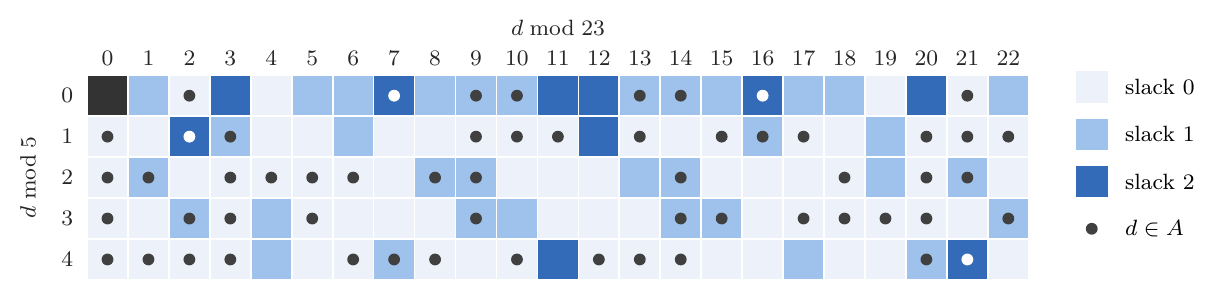
\includegraphics[width=0.92\textwidth]{figures/slack.png}
\caption{The slack $s(d)=59-3\ind{d\in A}-f(d)$ for $n=58$ at every $d\ne0$, with $d$ placed by its residues modulo $5$ and $23$; the black cell is $d=0$, and a dot marks $d\in A$. Equality holds for $70$ values of $d$, the slack is $1$ for $34$ and $2$ for $10$.}
\label{fig:slack}
\end{figure}

\section{Remarks}\label{sec:remarks}

\begin{remark}
The function $f$ is not constant on $A$ or on $C$ (Figure~\ref{fig:slack}): on the $58$ elements of $A$ it takes the values $54$, $55$ and $56$, for $4$, $18$ and $36$ of them, and on the $56$ elements of $C$ the values $57$, $58$ and $59$, for $6$, $16$ and $34$ of them. So the example is not a difference-set construction of the kind behind the infinite families in~\cite{Sz,Tu,We}.
\end{remark}

\begin{remark}
Unlike the graph for $n=67$ in~\cite{Bh}, this one has no multiplier symmetry beyond $d\mapsto-d$: the only units $u$ of $\Z_{115}$ with $uA=A$ are $\pm1$, the only one with $uB=B$ is $1$, and $B$ meets $-B$ in $29$ elements. So the $57$ rows of Table~\ref{tab:main} cannot be grouped into orbits as in~\cite{Bh}.
\end{remark}

\begin{remark}
We found the example by a computer search following the two-phase scheme of Turturean~\cite{Tu}. The first phase chooses $A$ so that the bounds $\NN_{B,B}(d)\le n+1-3\ind{d\in A}-\NN_{A,A}(d)$ leave a large margin in Fourier space, where they become linear conditions on the power spectrum of $B$. The second phase fixes $A$ and searches for $B$ by local search over exchanges of one element of $B$ with one outside it, guided by weights on the inequalities~\eqref{eq:star}; when no exchange lowers the weighted excess, the weights of the violated inequalities are raised, as in the breakout method of Morris~\cite{Mo}. No step of the proof above depends on the search.
\end{remark}

\begin{question}
The smallest open case of $R(B_{n-1},B_n)=4n-1$ is now $n=59$, with $v=117$; there $n$ is odd, and the regular two-block circulant graphs of~\cite{Bh,We} are available. Is there a two-block circulant graph over $\Z_{117}$, or over $\Z_3^2\times\Z_{13}$, that settles it?
\end{question}

\subsection*{Formal verification}
Theorem~\ref{thm:main} and the equality $R(B_{57},B_{58})=231$ are also proved in Lean~4~\cite{MU}, without any library beyond the Lean core. For the lower bound the development defines the graph $\Gamma(A,B)$ on the vertices $0,\dots,229$ by the two bit masks of $A$ and $B$, and the kernel evaluates the common neighbours and common non-neighbours of all $26{,}335$ pairs of vertices and checks that the adjacency is symmetric: every edge has at most $56$ common neighbours and every pair of distinct non-adjacent vertices has at most $57$ common non-neighbours. For the upper bound~\eqref{eq:RS} the development proves Goodman's count in the form used by Rousseau and Sheehan: if every edge of a graph on $N$ vertices lies in at most $a$ triangles and every non-edge has at most $b$ common non-neighbours, then counting the ordered triples of distinct vertices by the colours of their three pairs gives
\[
N(N-1)(N-2)\le\sum_{w}\bigl(3\,d(w)\,\bar d(w)+a\,d(w)+b\,\bar d(w)\bigr),
\]
where $d(w)$ is the degree of $w$ and $\bar d(w)=N-1-d(w)$. For $N=231$, $a=56$ and $b=57$ each term on the right is at most $230\cdot229$, with equality only when $d(w)=115$, and then the degrees would add up to the odd number $231\cdot115$. The final theorem states that $231$ is the least $N$ such that every graph on $N$ vertices contains $B_{57}$ or has a complement containing $B_{58}$; it depends only on the standard axioms \texttt{propext}, \texttt{Classical.choice} and \texttt{Quot.sound}. The graph is also checked by two independent programs, in Python and in C, which read the sets $A$ and $B$ and test all pairs directly. The development, the programs and the search are archived in~\cite{Ar}.

\subsection*{Use of generative AI}
The author used Claude (Anthropic) to search for the example, to check it by computer and in Lean, and to draft the text; the author verified every step and is responsible for the content.

\begin{thebibliography}{99}

\bibitem{Ar}
D.~Bhattacharjee, \emph{Book Ramsey numbers $R(B_{57},B_{58})=231$ and $R(B_{66},B_{67})=267$: data, checks, search and Lean~4 proofs}, Zenodo, 2026, all versions \doi{10.5281/zenodo.23373628}. Source code at \url{https://github.com/creelie/Breakthrough-problems-2}

\bibitem{Bh}
D.~Bhattacharjee, \emph{A hand-checkable proof that $R(B_{66},B_{67})=267$}, preprint, 2026, archived in~\cite{Ar}.

\bibitem{CDW}
S.~Chung, W.~Du and W.~J.~Wesley, \emph{Autonomous mathematical discovery in an open-world multi-agent environment}, preprint, 2026. \href{https://arxiv.org/abs/2608.23691}{arXiv:2608.23691}

\bibitem{CDWd}
S.~Chung, W.~Du and W.~J.~Wesley, \emph{Station data v2}, book Ramsey verification notebook and certificates, first public version 24 August 2026. \url{https://github.com/dualverse-ai/station_data_v2}, accessed 14 October 2026.

\bibitem{Ep}
Epoch AI, \emph{FrontierMath open problems: Ramsey numbers for book graphs}, 2026. \url{https://epoch.ai/frontiermath/open-problems/ramsey-book-graphs}, accessed 15 October 2026.

\bibitem{Go}
A.~W.~Goodman, \emph{On sets of acquaintances and strangers at any party}, Amer. Math. Monthly \textbf{66} (1959), no.~9, 778--783. \doi{10.1080/00029890.1959.11989408}

\bibitem{MU}
L.~de~Moura and S.~Ullrich, \emph{The Lean~4 theorem prover and programming language}, in: Automated Deduction -- CADE~28, Lecture Notes in Comput. Sci. \textbf{12699}, Springer, Cham, 2021, 625--635. \doi{10.1007/978-3-030-79876-5_37}

\bibitem{Mo}
P.~Morris, \emph{The breakout method for escaping from local minima}, in: Proceedings of the Eleventh National Conference on Artificial Intelligence (AAAI-93), AAAI Press, 1993, 40--45. \url{https://cdn.aaai.org/AAAI/1993/AAAI93-007.pdf}

\bibitem{RS}
C.~C.~Rousseau and J.~Sheehan, \emph{On Ramsey numbers for books}, J. Graph Theory \textbf{2} (1978), 77--87. \doi{10.1002/jgt.3190020110}

\bibitem{Sz}
G.~Szekeres, \emph{Tournaments and Hadamard matrices}, Enseign. Math.~(2) \textbf{15} (1969), 269--278.

\bibitem{Tu}
D.~Turturean, \emph{Summary of new results on the Ramsey numbers for book graphs open problem}, 2026. \url{https://docs.google.com/document/d/1VinXOiMov2v-Y27GTJwoAECywv2a34MH4E8qa712zJY}

\bibitem{We}
W.~J.~Wesley, \emph{Lower bounds for book Ramsey numbers}, Discrete Math. \textbf{349} (2026), no.~5, 114913. \doi{10.1016/j.disc.2025.114913}

\end{thebibliography}

\end{document}
